\documentclass[11pt,xcolor=svgnames]{beamer}
\usepackage{dsfont,natbib,setspace,changepage,multirow}
\mode<presentation>

% replaces beamer foot with simple page number
\setbeamertemplate{navigation symbols}{}
%\setbeamerfont{frametitle}{series=\bfseries}
\setbeamercolor{frametitle}{fg=Black}

\setbeamertemplate{footline}{
   \raisebox{5pt}{\makebox[\paperwidth]{\hfill\makebox[20pt]{\color{gray}\scriptsize\insertframenumber}}}}

\graphicspath{{/Users/mtaddy/Dropbox/inputs/}}
\usepackage{algorithm}
\usepackage{algorithmic}

% colors
\newcommand{\theme}{\color{Maroon}}
\newcommand{\bk}{\color{black}}
\newcommand{\rd}{\color{DarkRed}}
\newcommand{\fg}{\color{ForestGreen}}
\newcommand{\bl}{\color{blue}}
\newcommand{\gr}{\color{black!67}}
\newcommand{\sg}{\color{DarkSlateGray}}
\newcommand{\nv}{\color{Navy}}
\setbeamercolor{itemize item}{fg=gray}

% common math markups
\newcommand{\bs}[1]{\boldsymbol{#1}}
\newcommand{\mc}[1]{\mathcal{#1}}
\newcommand{\mr}[1]{\mathrm{#1}}
\newcommand{\bm}[1]{\mathbf{#1}}
\newcommand{\ds}[1]{\mathds{#1}}
\newcommand{\indep}{\perp\!\!\!\perp}
\def\plus{\texttt{+}}
\def\minus{\texttt{-}}

% spacing and style shorthand
\setstretch{1.1} 

\begin{document}

\setcounter{page}{0}
{ \usebackgroundtemplate{\includegraphics[height=\paperheight]{phoenix}}
\begin{frame}[plain]
\begin{center}


{\bf \Large Document Classification by Inversion of \\Distributed Language Representations}

\vskip 1cm\large
 Matt Taddy,  Chicago Booth

\end{center}
\end{frame} }

\begin{frame}


{\bf Distributed language representation}

\vskip .5cm
$\theme  \boldsymbol{\mathcal{V}}$ contains
an embedding  in $\mathds{R}^K$ for every vocabulary  word.

\vskip .25cm
In a contextual language model, $\mathcal{V}$ is trained to maximize the likelihoods for each single words and its neighbors.  

\vskip .25cm
e.g., The {\theme skip-gram} objective for word $t$ in sentence $s$ is
\begin{equation*}\label{eq:skipgram}
\mathrm{max}\sum_{j\neq t,~j=t-b}^{t+b} \log\mathrm{p}_{\mathcal{V}}(w_{sj}\mid w_{st})
\end{equation*}
where $b$ is the skip-gram window (truncate at ends of sentences).

\end{frame}

\begin{frame}

{\bf Neural network language models}

\vskip .5cm
Local context probabilities are functions of the word embeddings.

\vskip .25cm
e.g., In {\theme Word2Vec} {\gr (Mikolov et al. 2013)}
\begin{equation*} \label{eq:neuralnet}
\mathrm{p}_{\mathcal{V}}(w | w_t) =
 \prod_{j=1}^{L(w)-1}\sigma\!\left( \mathrm{ch}\left[\eta(w,j+1)\right] \mathbf{u}_{\eta(w,j)}^\top \mathbf{v}_{w_t} \right) 
\end{equation*}
where $\eta(w,i)$ is the $i^{th}$ node in the length-$L(w)$ Huffman tree path for  $w$ and $\mathrm{ch}(\eta)
\in \{-1,+1\}$ for whether $\eta$ is a left or right child.

\vskip .25cm
\gr `Output' embedding $\mathbf{v}_{w_t}$ is usually the main object of interest.
\end{frame}


% \begin{frame}

% {\bf Example Huffman encoding of a 4 word vocabulary}

% \begin{center}
% 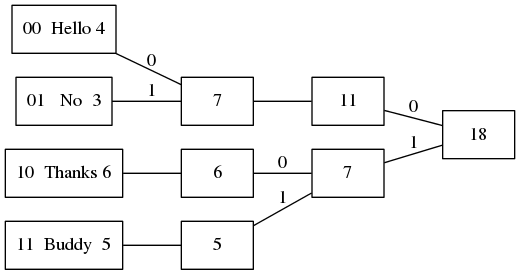
\includegraphics[width=.9\textwidth]{graphs/bht}
% \end{center}

% From left to right the two nodes with lowest count are
% combined into a parent.  Encodings are read off of the splits
%  from right to left. 

% \end{frame}

\begin{frame}

{\bf From word embeddings to document modeling}

\vskip .5cm
Distributed representations have proven very useful for NLP tasks {\gr next word prediction, word analogy, named entity recognition, ...}

\vskip .25cm 
There is interest in porting this success to document modeling
{\gr author classification, sentiment prediction, attribute imputation, ...}

\vskip .35cm 
Strategies include directly modeling the semantic composition of contexts {\gr (Socher et al. 2011)} or adding latent document-location effects into the context model {\gr (as in Le \texttt{+} Mikolov's Doc2Vec)}.

\vskip .5cm
{\theme This paper:} composite likelihoods and Bayes rule provide a very simple way to turn local language models into document classifiers.
\end{frame}


\begin{frame}

{ \bf Composite likelihood}
\vskip .5cm

The local-context objectives don't correspond to a full document model, but they can be combined to form a composite likelihood.

\vskip .25cm
e.g., skip-gram's pairwise-conditional composition for sentence $\bm{w}$
\begin{equation*}\label{eq:sentencelhd} \log\mathrm{p}_{ \mathcal{V}}(\mathbf{w}) = 
\sum_{j=1}^T\sum_{k=1}^T \mathds{1}_{\left[1\leq |k-j| \leq b\right]} \log\mathrm{p}_{ \mathcal{V}}(w_{k}|
w_{j} ). \end{equation*} 

{\theme Composite LHD approximate a full joint LHD}. They are common in  statistics, since Besag's  pseudolikelihood $\mathrm{p}(\mathbf{w}) \approx \prod_j \mathrm{p}(w_j |\mathbf{w}_{-j})$.

\vskip .25cm
{\gr Another e.g.: Jernite et al. (2015) show that CBOW Word2Vec corresponds to the pseudolikelihood for a Markov random field.  }

\end{frame}

\begin{frame}

{ \bf Bayesian inversion}
\vskip .5cm

Given sentence LHDs, document $d =
\{\mathbf{w}_1, ... \mathbf{w}_S\}$ has  log LHD 
\begin{equation*}\label{eq:fulllhd} \log\mathrm{p}_{ \mathcal{V}}(d) = 
\sum_{s}  \log\mathrm{p}_{ \mathcal{V}}(\mathbf{w}_s). \end{equation*} 

\vskip .2cm
{Suppose your documents are grouped by class label, $y \in
\{1 \dots C\}$.}  

\vskip .1cm
{\theme Then you train separate $\mathcal{V}_c$ on each sub-corpus $D_c = \{ d_i : y_i =c \}$.}

\vskip .1cm
$\Rightarrow$ doc $d$ has probability
$\mathrm{p}_{ \mathcal{V}_c}(d)$ if it came from class $c$, and
\begin{equation*}\label{eq:bayesrule}
\mathrm{p}( y | d) = \frac{\mathrm{p}_{ \mathcal{V}_y}(d)\pi_y }
{\sum_c \mathrm{p}_{ \mathcal{V}_c}(d)\pi_c }
\end{equation*}
where $\pi_c$ is our prior probability on class label $c$ {\gr (say $\pi_c = 1/C$)}.


\end{frame}


\begin{frame}

{\bf Yelp reviews example}

\vskip .25cm
200k reviews, 2mil sentences, separate W2V for each of 1-5 stars.

\vskip .25cm
Given W2V representations $\mathcal{V}_1 \ldots \mathcal{V}_5$, calculate sentiment probs as, e.g.,
$\mathrm{p}(\star \geq 3|d) = \left[\mathrm{p}_{ \mathcal{V}_3}(d) +
\mathrm{p}_{ \mathcal{V}_4}(d) +
\mathrm{p}_{ \mathcal{V}_5}(d) 
\right]/
{\sum_{c=1}^5 \mathrm{p}_{ \mathcal{V}_c}(d) }$
\begin{center}
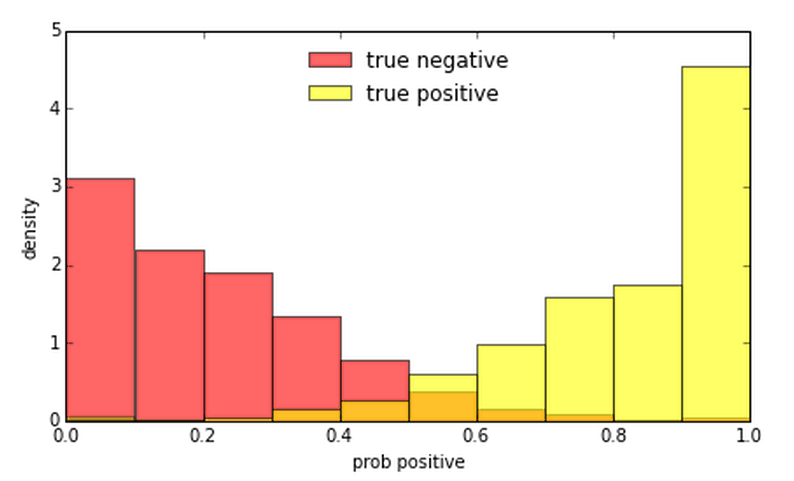
\includegraphics[width=0.6\textwidth]{graphs/posneg}
\end{center}

% {\footnotesize
% $\star \geq 3$: very yummy food, friendly staff, quick service, and good coffee.

% $\star < 3$: went for lunch. the place smelled bad, like cig smoke. we ordered but  were told that they didnt have food.}

Everything is implemented in the \texttt{gensim} library for \texttt{python}, which now includes the \texttt{score} method to obtain $\log \mathrm{p}_{ \mathcal{V}}(d)$ for fitted $\mathcal{V}$.

\end{frame}

\begin{frame}


{\bf OOS classification performance}

\begin{center}
{\footnotesize
 \begin{tabular}{r|c|c|c}
{\it misclass rate} & $<,\geq 3 ~\star$ & $<,=,>3$ $\star$ &  $1 \dots 5 ~\star$
\\ \cline{1-4}\rule{0pt}{3ex}
W2V inversion & .099 & \textbf{.189} & .435 \\
Phrase regression & \textbf{.084} & .200 & \textbf{.410} \\
%D2V DBOW &  .144 &.282 & .496 \\
%D2V DM & .179 & .306 & .549 \\
D2V combined & .148 & . 284 & .500 \\
MNIR & .095 & .254 & .480 \\
W2V aggregation & .118 & .248 & .461 
\end{tabular}}
\end{center}

\begin{center}
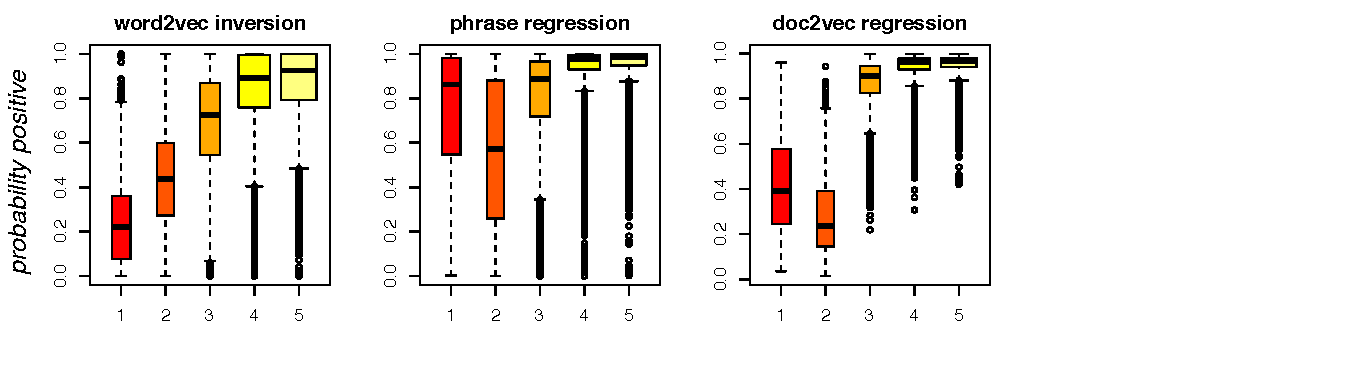
\includegraphics[width=1\textwidth]{graphs/bystarshort}
\end{center}

Best or close to it, with prob(\textit{positive}) nicely ordered by true star.
\end{frame}



\begin{frame}

{\bf Inversion is simple, scalable, and it works}

\vskip .5cm
Not claiming it's a world beater, but it is an easy way to go from a context representation algorithms to document classification.

\vskip .5cm
{\gr Future questions...}

\vskip .25cm
Can we use what we know about composite LHD to drive  context models? {\gr e.g., Cox \texttt{+} Reid (2004): $\mathrm{p}(w_j,w_k)$ pref to $\mathrm{p}(w_j|w_k)$.}

\vskip .25cm
Given the local $\rightarrow$ global connection, can we apply distributed representations in new domains? {\gr e.g., consumer product choices.}

\vskip 1cm
\hfill{\bf \LARGE \theme THANKS!}

\end{frame}

\end{document}






























